\documentclass{jreport}

\usepackage{amsmath,amsthm}
\usepackage{amssymb}
\usepackage{multicol}
\usepackage[dvipdfmx]{graphicx}
\usepackage[top=25truemm,bottom=20truemm,left=20truemm,right=20truemm]{geometry}
\usepackage{wrapfig}
\usepackage[all]{xy}
\def\objectstyle{\displaystyle}

\theoremstyle{idefinition} 
\newtheorem{idefi}{定義}[section] 
\newtheorem{iqst}[idefi]{問題} 
\newtheorem{iprop}[idefi]{命題} 
\newtheorem{ithm}[idefi]{定理}  
\renewcommand\proofname{\bf 証明} 

 



\begin{document}

\chapter{正多面体(井上)}

\section{前書き}
\ こんにちは、数学科の井上です.今年で4年生なので,e$\pi$isodeの原稿を書くのも今回が最後となります.といっても3年の時は少し展示を手伝ったのみなので,寄稿するのは2回目なのですけれど.e$\pi$isodeのメインのターゲットの読者は中高生ですので,読んで数学っておもしろいなと思ってもらえるものを書けたらいいなと思ってます.難しいことはきっと誰かが書いてくれるので私は書きません.(書けません?)少しでも興味をもって読んでもらえれば嬉しいです.\\

\section{正多面体}
\begin{idefi}
\ 正多面体(orプラトンの立体)とは,すべての面が同一の正多角形で構成され,すべての頂点で接する面の数が等しい凸多面体のこと.
\end{idefi}

\begin{ithm}
\ 正多面体は正四面体,正六面体,正八面体,正十二面体,正二十面体の$5$つのみである.
\end{ithm}

\ 正多面体が5つしかないことは有名なので,証明も含めてご存知の方も多いと思います.一つだけ証明を紹介します.ほかにもオイラーの多面体公式((頂点の数)$-$(辺の数)$+$(面の数)$=2$)を用いても示せます.\\

\begin{proof}
\ 多面体を構成する多角形を正$n$角形とし,頂点に集まる面の数を$m$個とします.このとき正多角形の角の大きさは$\frac{(n-2)\pi}{n}$なので,各頂点に集まる角度の和は$\frac{m(n-2)\pi}{n}$となる.凸多面体であるために,各頂点に集まる角の和は$2\pi$未満であることが必要になる.よって$\frac{m(n-2)\pi}{n}<2\pi$という式が得られる.
\[
\begin{array}{ccc}
\frac{m(n-2)\pi}{n}<2\pi & \Longleftrightarrow & mn-2n-2m<0 \\
& \Longleftrightarrow & \frac{1}{n}+\frac{1}{m}>\frac{1}{2}\\
\end{array}
\]
\ $n,m$は定め方から$n,m\leq3$を満たす整数であることに注意すると条件を満たすのは$(n,m)=(3,3),(3,4),(3,5),(4,3),(5,3)$の$5$通り.これらはそれぞれ正四面体,正八面体,正二十面体,正六面体,正十二面体になっている.
\end{proof}

\ なぜ正多面体の話をしようと思ったのか少し動機を説明しますと,定義からも分かるように正多面体は非常に対称性の高い立体です.この対称性がいろいろなところに顔を出していて面白いからです.正多面体を自分自身に移す合同変換を通して対称性を考えます.\\

\newpage

\begin{wrapfigure}{r}{10cm}
\vspace{-4\baselineskip}
\begin{center}
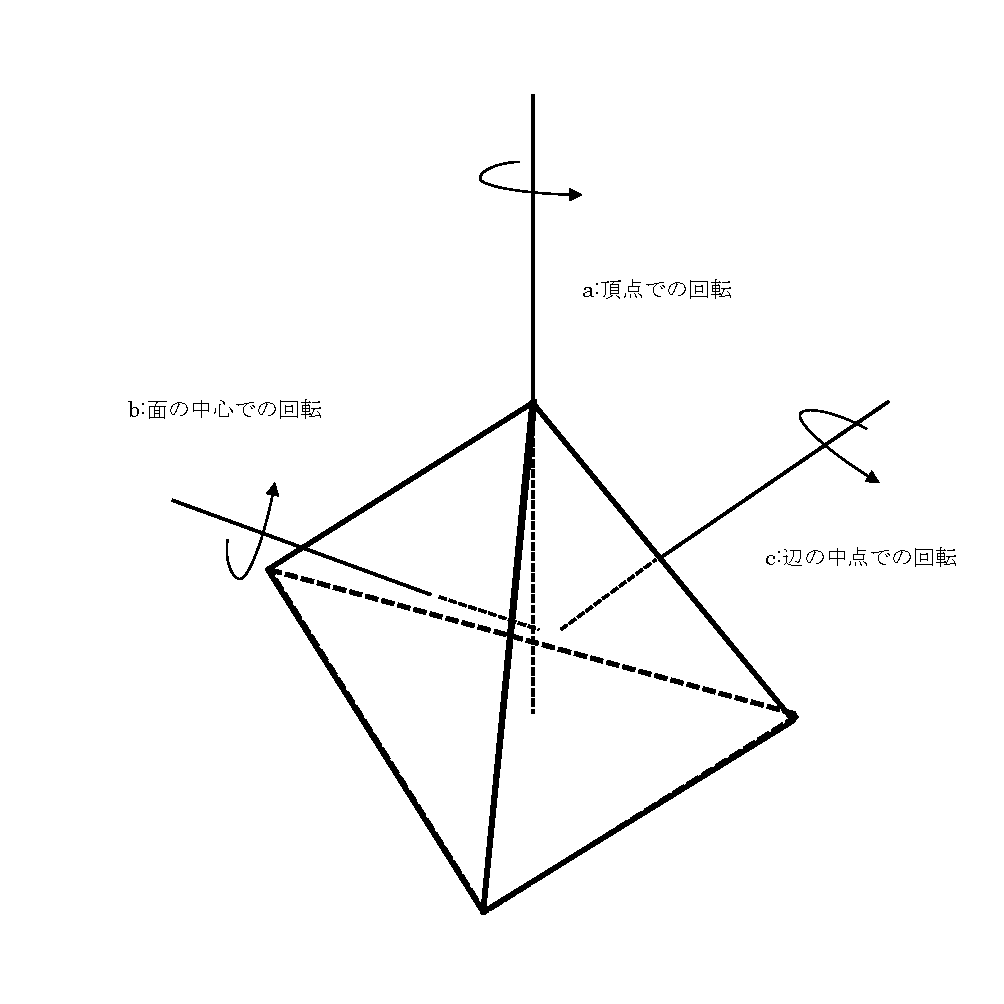
\includegraphics[width=10cm]{i1.pdf}
\end{center}
\vspace{-3\baselineskip}
\end{wrapfigure}


\ 一番単純な正四面体を例にとって対称性を見ていきます.\\
\ このとき右の図のように,頂点における回転と,面の中心における回転,辺の中点における回転の$3$つが考えられます.まず頂点の回転については$\frac{2\pi}{3},\frac{4\pi}{3}$回転したときに,元の図形にぴったり重なります.これを4つの各頂点で考えます.次に面の中心の回転についても$\frac{2\pi}{3},\frac{4\pi}{3}$回転したときに,元の図形にぴったり重なりますが,実はこれは頂点での回転を反対側から見ただけの操作になっています.つまり,頂点での回転と同一視されます.最後に辺の中点での回転ですがこれは$\pi$回転のみで,ある辺の中点での回転とそれと向かい合う辺の中点での回転は同一のものになっています.つまり辺の数は6本ですが,辺3本分のみ考えます.また,何も動かさないという操作も一つの操作として数に入れます.\\
\ これらの結果を合わせると全部で,$1+4\times2 +3 \times 1 =12$通りの形を保つ回転の操作があることが分かります.この操作たちを回転による対称性の群とよびます.\\


\begin{idefi}
\ 正$k$面体に対して,その回転による対称性の群を$k$面体群という.さらに,鏡映を含めた対称性の群を拡大$k$面体群という.
\end{idefi}

\ $k$面体群や拡大$k$面体群が確かに群になっていることは少し確認すればわかります.(ちなみに入っている演算は,回転・鏡映等の操作の合成です.)一応群の定義を次にあげておきますが,特別な集合だと思っても本稿を読む上ではさしつかえありません.\\

\begin{idefi}
\ 集合$G$とその上の演算$\cdot$が群であるとは,以下を満たすこと.\\
\ 任意の$g,h,k \in G$について,\\
\ 1. 結合法則$g\cdot(h\cdot k)=(g\cdot h)\cdot k$を満たす\\
\ 2. $g\cdot 1=1 \cdot g=g$となる単位元$1$が存在する\\
\ 3. $g\cdot g^{-1}=g^{-1}\cdot g=1$となる逆元$g^{-1}$が存在する\\
\end{idefi}


\ 正多面体のそれぞれの特徴をあげると次のようになります.\\


\begin{tabular}{|c||c|c|c|c|c|c|}\hline
正k面体 & 面の種類(正n角形) & 面の数 & 頂点の数 & 辺の数 & k面体群の位数(元の数) & k面体群と同型な群\\\hline
4 & 3 & 4 & 4 & 6 & 12 & $\mathfrak{A}_4$\\\hline 
6 & 4 & 6 & 8 & 12 & 24 & $\mathfrak{S}_4$\\\hline 
8 & 3 & 8 & 6 & 12 & 24 & $\mathfrak{S}_4$\\\hline 
12 & 5 & 12 & 20 & 30 & 60 & $\mathfrak{A}_5$\\\hline 
20 & 3 & 20 & 12 & 30 & 60 & $\mathfrak{A}_5$\\\hline 
\end{tabular}\\

\ $k$面体群の位数に関しては,四面体群の時と同様に頂点における回転と,面の中心における回転,辺の中点における回転の$3$つを重複のないように数え上げれば求められます.\\
\ 正六面体と正八面体,正十二面体と正二十面体,いずれも$k$面体群が同型になっています.これはこの二組がそれぞれ双対と呼ばれる関係になっていることと関係があります.ここでは2つの多面体が双対であることを一方の多面体の辺の中心を結んだらもう一方の多面体になるということで定義します.\\
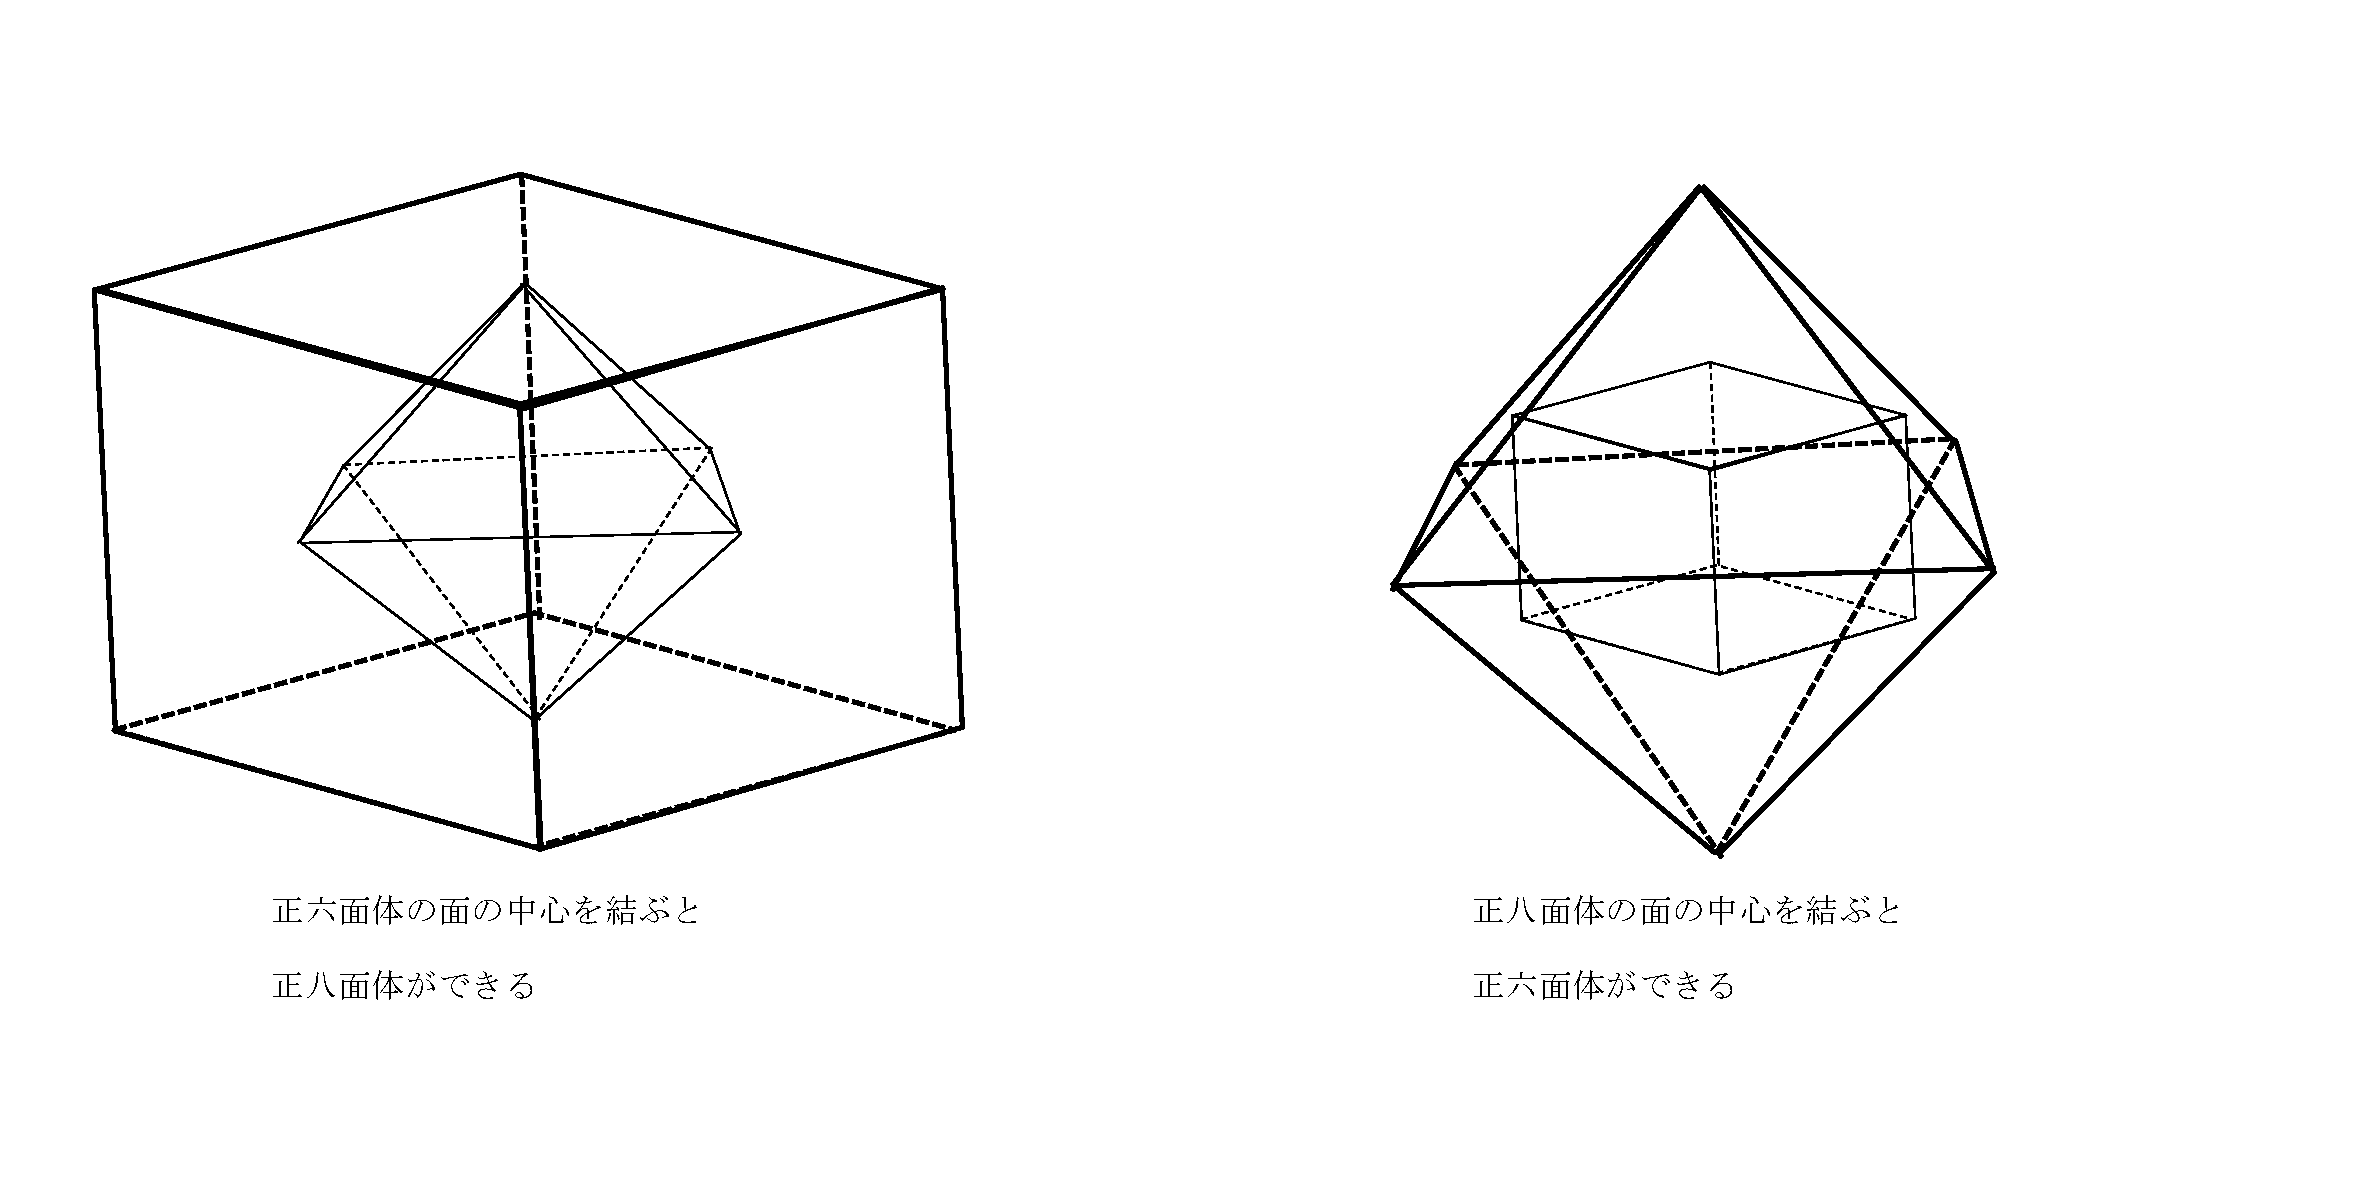
\includegraphics[width=18cm]{i2.pdf}\\
\ 双対な多角形同士では,それぞれ頂点における回転と面の中心における回転が1対1に対応しているので,回転による対称性を考えると同じ対称性を持っていることがわかります.\\



\section{対称群}
\ 前節の表に出てきた$\mathfrak{S}_4$や$\mathfrak{A}$について説明をします.($\mathfrak{A}$はAを,$\mathfrak{S}$はSをフラクトゥール文字で書いたものです.慣習的にこう書かれます.)まず$\mathfrak{S}_n$について.この$n$には正の整数が入ります.これは$1,2,\cdots,n$の順に並んでいた$n$個の数字を並べ替える操作全体によってできる群を表しています.$k$と$l$を入れ替える操作のことを$(kl)$と書きます.例えば$n=3$のとき,
\[
\begin{array}{cccll}
123&\rightarrow&123&何もしない&id(恒等写像)と書く\\
123&\rightarrow&132&2と3を入れ替える&(23)と書かれる\\
123&\rightarrow&213&1と2を入れ替える&(12)と書かれる\\
123&\rightarrow&231&1と2を入れ替えた後2のあった場所にある1と3を入れ替える&(12)(23)と書かれる\\
123&\rightarrow&312&1と2を入れ替えた後1のあった場所にある2と3を入れ替える&(12)(13)と書かれる\\
123&\rightarrow&321&1と3を入れ替える&(13)と書かれる\\
\end{array}
\]
\ よって$\mathfrak{S}_3=\{id,(12),(13),(23),(12)(13),(12)(23)\}$となることがわかります.(12)(23)を3つの数の入れ替えとみなして(123)という書き方をすることもあります.(kl)のように2つの数を入れ替えているものを互換といいます.実は$\mathfrak{S}_n$の元は全て互換の積の形で書き表すことができます.\\

\begin{idefi}
\ $\mathfrak{S}_n$の元を互換の積で書き表したとき,偶数個の互換の積で書き表せるものを偶置換といい,奇数個の互換の積で表せるものを奇置換という.このとき偶置換全体の集合を$\mathfrak{A}_n$と書く.
\end{idefi}

\ 四面体群が$\mathfrak{A}_4$とみなせるのはどうしてでしょう.四面体の頂点に1~4の番号を振ります.すると回転というのはこの四面体の番号を入れ替えることに他なりません.例えば頂点を中心にして$\frac{2\pi}{3}$回転させることを考えます.\\
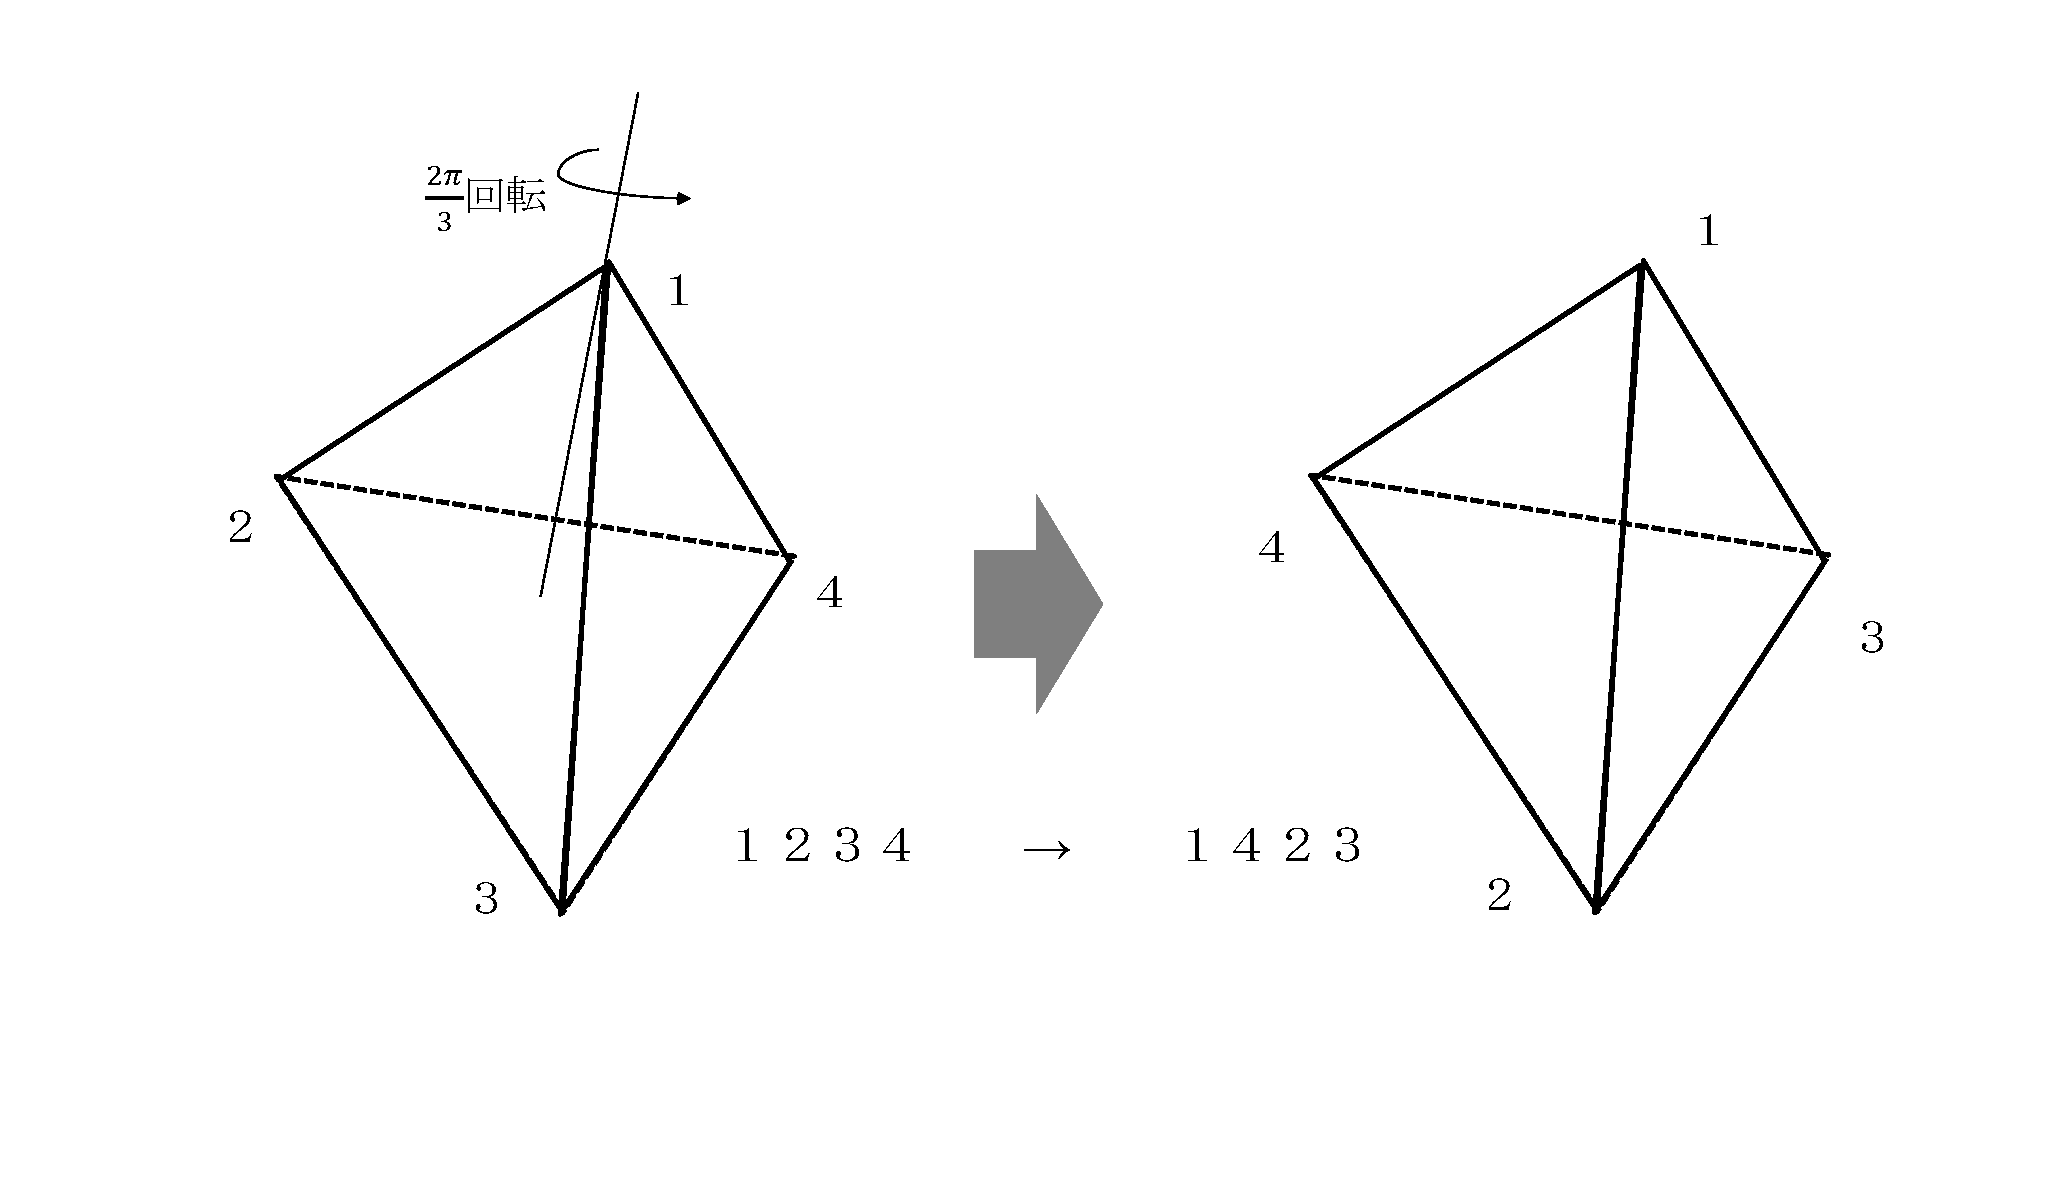
\includegraphics[width=15cm]{i3.pdf}\\
\ 上の図のように回転をさせることと頂点を入れ替えることが対応しています.ここで$1234\rightarrow1423$というのは(24)(34)に対応しています.ほかの回転も全て試してみると,この四面体の対称性の群がちょうど$\mathfrak{A}_4$に一致することがわかります.ちなみに鏡映も含めた拡大四面体群のほうは$\mathfrak{S}_4$に一致します.\\

\ ほかの多面体についても,同様に考察ができますが番号を振り方をうまく工夫する必要があります.例えば,正六面体群は$\mathfrak{S}_8$よりずいぶん小さいですから,頂点に全部に番号を振ったものを考えても仕方ありません.(一般に$k\leq l$のとき$\mathfrak{S}_k \subset \mathfrak{S}_l$であることは定義からわかるので,確かに$\mathfrak{S}_4 \subset \mathfrak{S}_8$になりますが.)この場合は一番離れた所にある頂点同士の関係はいくら回転させても変わらないことを利用します.すると半分の数の頂点に番号を振れば十分ということがわかります.\\

\section{Mckay理論}
\ これから書くのはおまけの話です.まともに説明すると紙面が足りなくなるので,厳密性のないただのお話として紹介します.Mckay対応といって,今まで散々見てきた多面体群と単純リー環のルート系という数学的に興味のある対象を,一対一に対応させるおもしろい理論があります.リー環がなんであるかについては,足し算とある種の積の入った環でそこそこ扱いやすいものだと思ってください.\\
\begin{ithm}
\ $2$次元特殊線形群$SL(2)$の有限部分群は次の5つのいずれかに同型になる.\\
\ 位nlの巡回群$(A_{n-1})$\\
\ 多面体群:正二面体群$(D_{n+2})$,正四面体群$(E_6)$,正八面体群$(E_7)$,正二十面体群$(E_8)$\\
\ ただし$n \in\mathbb{N}_{ \geq 2}$とする.
\end{ithm}
\ $2$次元特殊線形群$SL(2)$とは行列群の一種で,
\begin{eqnarray*}
SL(2)&=&\{X\in GL(2,\mathbb{C}) | \det X=1\}\\
&=&\{
\begin{pmatrix} 
a&b\\ 
c&d\\ 
\end{pmatrix}
| a,b,c,d \in \mathbb{C} ,ad-bc=1\}
\end{eqnarray*}
\ で定義されます.\\
\ 位数nの巡回群についてですが,これは正$n$角形に対する回転による合同変換が作る群と同一視できます.一方,正二面体群は正$n$角形に対する回転と鏡映による合同変換が作る群と同一視できます.\\
\ この群$G$の持つ性質を知りたいと思ったときに,表現というものを考えてこれにより$G$を特徴づけようという考え方があります.\\

\begin{ithm}(Macky)
\ $SL(2,\mathbb{C})$の有限部分群Gの表現から構成されるディンキン図形は,既約ルート系のsimply laced (辺がすべて一本線である) といわれるディンキン図形と同型である.
\end{ithm}
\ 既約ルート系のディンキン図形が単純リー環と一対一に対応しています.そのため単純ではないリー環にも同様の対応があるのではないかと研究がすすめられています.\\

\ ディンキン図形は表現やルート系などから一意的に構成できますが,次のようなものです.\\
\[A_{n-1}型 : 
\underbrace{
\xymatrix@!C{
\circ \ar@{-}[r] & \circ \ar@{-}[r] & \cdots \ar@{-}[r] & \circ \ar@{-}[r] & \circ
}
}_{n-1個}
\]
\[D_{n+1}型 : 
\underbrace{
\xymatrix@!C{
&&&\circ \ar@{-}[d]&\\
\circ \ar@{-}[r] & \circ \ar@{-}[r] & \cdots \ar@{-}[r] & \circ \ar@{-}[r] & \circ
}
}_{n+1個}
\]
\[E_6型 : 
\xymatrix@!C{
&&\circ \ar@{-}[d]&&\\
\circ \ar@{-}[r] & \circ \ar@{-}[r] & \circ \ar@{-}[r] & \circ \ar@{-}[r] & \circ
}
\]
\[E_7型 : 
\xymatrix@!C{
&&\circ \ar@{-}[d]&&&\\
\circ \ar@{-}[r] & \circ \ar@{-}[r] & \circ \ar@{-}[r] & \circ \ar@{-}[r] & \circ \ar@{-}[r] & \circ
}
\]
\[E_8型 : 
\xymatrix@!C{
&&\circ \ar@{-}[d]&&&&\\
\circ \ar@{-}[r] & \circ \ar@{-}[r] & \circ \ar@{-}[r] & \circ \ar@{-}[r] & \circ \ar@{-}[r] & \circ \ar@{-}[r] & \circ
}
\]

\section{参考文献}
\ 『表現論入門セミナー』,平井武・山下博,遊星社(2003)\\
\ 『鏡映の数学 : 有限鏡映群の幾何学』 A.V.ボロビック, A.ボロビック著 ; 小林雅人 [ほか] 訳,丸善出版(2015)\\
\ 『特異点とルート系』 松澤淳一著,朝倉書店(2002)\\








\end{document}
